\documentclass[Main]{subfiles}
\begin{document}

\subsection{Planning procedure}

The proposed planning procedure for a multi-agent system can be divided in to "??????? four ????????" algorithms. The first being the distribution of goals between agents, done with a bidding algorithm. 
The \textit{bidding algorithm} utilizes simple heuristics consisting of the Manhattan distance between an agent and box, and box and goal, with a slight favoring of as few box moves as possible. All agents in the level will bid on all goals, that it is eligible for solving, and it will do so for all boxes that can solve the goal. After a round of bidding, the smallest bid, in terms of heuristics, is evaluated in order to determine if it is possible for the agent to fulfill the bid. The evaluation is done as a relaxed problem search. 

If the relaxed problem search returns a valid plan for the solving the goal, the agent will win the bid and the goal will be assigned to the agent. The relaxed plan, among others, containing information about goal, box, agent and traveled path, is kept and used for further preprocessing. 
When a box is used for solving a relaxed plan, it will be marked as such, and bids on other goals, using that same box, will be ignored. 

Should an agent not be able to fulfill a bid, the next best bid will be chosen and evaluated, and so on. 





- If not feasible - next bid
- If agent is "overburdened" - next bid
- If box is used

%\cite{BIDDING - SOMETHING from bjarke}
\cite{van2005coordination}


The \textit{relaxed problem search} regards the level with only one agent at its initial location, one goal and one box that can possibly solve the goal. The search is done with $A^*$ strategy. 

The relaxed problem search also functions as a sort of ``all goals shortest path'' calculation. It is however, not the shortest paths for all goals, but while it might be for some, it shows a possible path for all goals. 


\textit{Other advantages of relaxed problem search}

The relaxed problem search finds a possible solution for all goals, which provide valuable information about the level for preprocessing. 





\subsubsection{Goal ordering}

- Regarding conflicts


- Regarding plan size - from initial location


\textit{Conflicts and constraints}

Conflicts between goals, meaning solved goals that will block agents from moving to other goals, is used for determining ordering constraints for the final goal solving algorithm. 

Conflicts are defined as goals cells, other than the goal being solved, that an agent has to move through with a box, in order to solve a goal. The path from the solution to the relaxed problem is used for this check. This approach has some drawbacks, one being, that maybe the agent could just move the box in a cell next to the goal, like the case below: \\

\begin{figure}[h!]
    \centering
    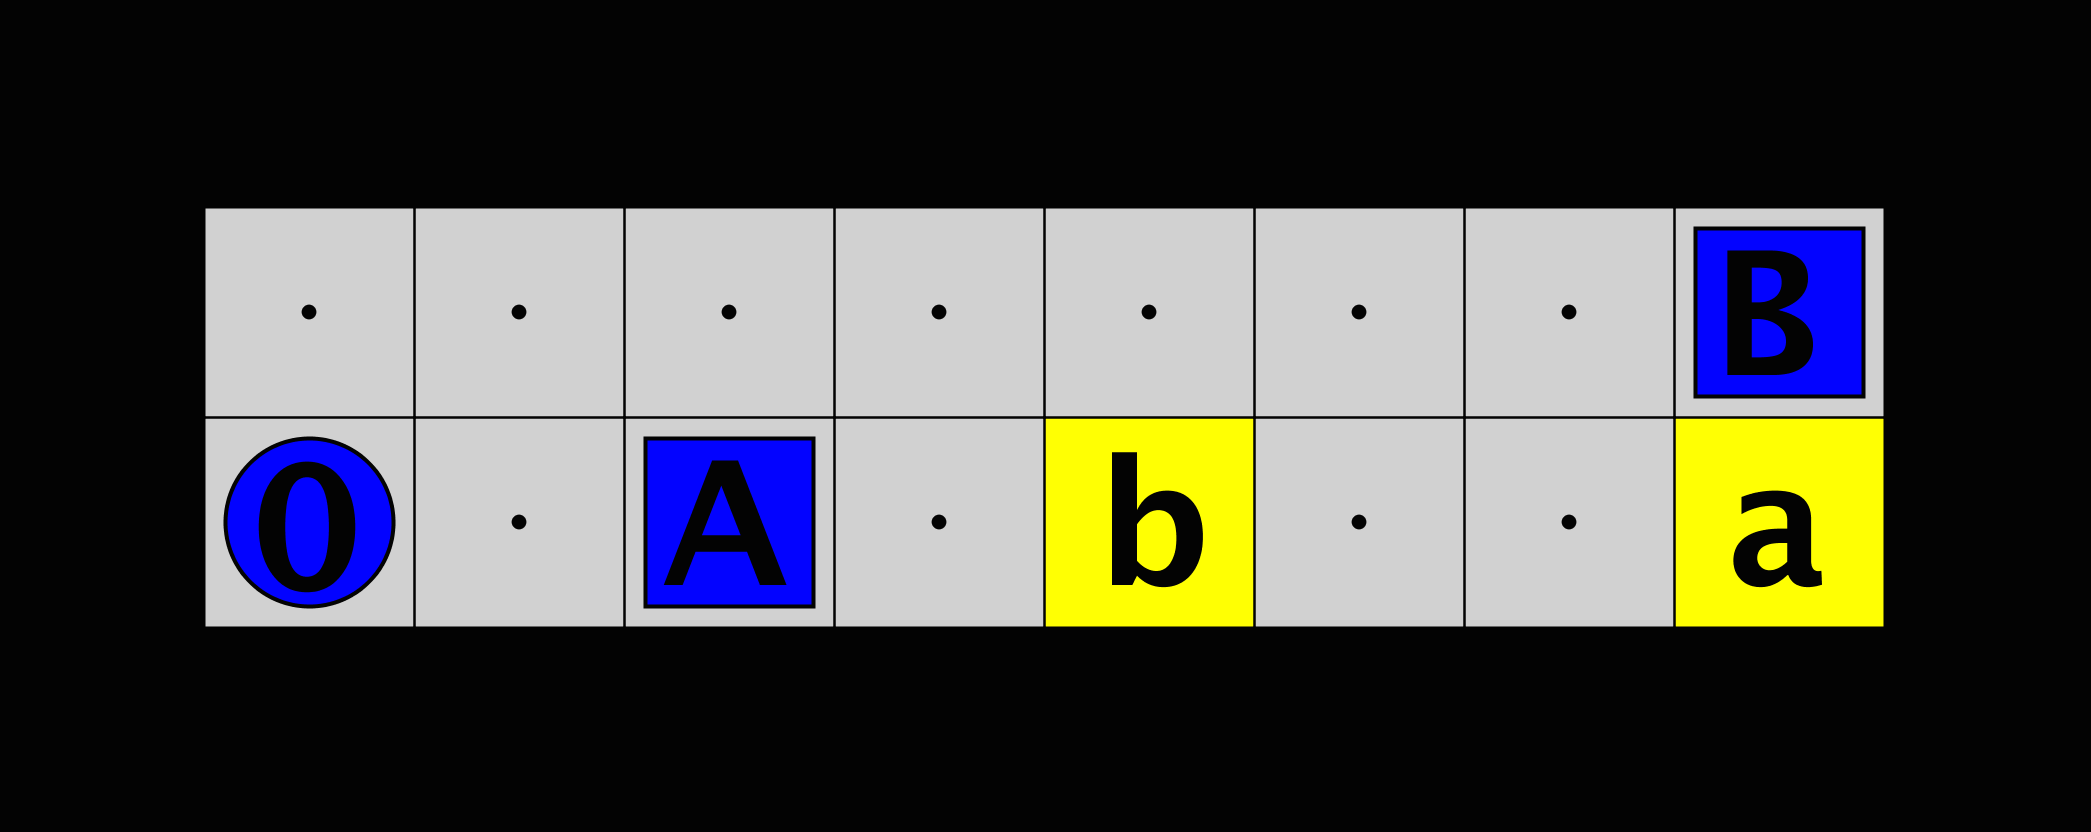
\includegraphics[width=0.3\textwidth]{conflict.png}
    \caption{Case that can be seen as a conflict, but can be avoided}
    \label{fig:conflict_avoidable}
\end{figure}

% \begin{verbatim}
% ++++++++++
% +       B+
% +0 A b  a+
% ++++++++++
% \end{verbatim}

In this case, the solution to the relaxed problem, will involve the agent pushing box ``A'' through the goal ``b''. This is however not a real conflict, as the agent could just move the box around the goal ``b'', should it already be solved at the time it is solving ``a''. A simple way of trying to avoid this, is to do a check on the cells surrounding the goal. 
The conflict found in the case above will be determined as being avoidable, and hereby not trigger any ordering constraint between goal ``a'' and ``b''. 



\textit{Size prioritizing} - Redundant ??

THe length of the solution to the relaxed problem is used for prioritizing goals.



\textit{Summary}

Sorting of the goals is done with a comparing algorithm with two factors, being ordering constraints and solution size. The ordering constraints always have the highest priority, such that if there exists a conflict between two goals, the goal cell that blocks for the solution of another goal will have to be solved after the goal who's path it is blocking. If there are no mutual conflicts between to goals, the one with the shortest solution to the relaxed problem will be prioritized before the other. 




\subsubsection{Backtracking}




\subsection{POP - rename or move this ``?????'' }
Partial order planning can be said to occur twice in the planning procedure, as the procedure consists of two major parts. The first part is a sort of ``all goals shortest path'' calculation as well as a determination of goal ordering / prioritizing. 
It is done as a relaxed problem search where the only components regarded are the goal to be solved, a box to solve it with, the agent to move the box, and the walls of the level. The relaxed problem is solved utilizing A\^{*} search strategy. 





\subsubsection{Heuristics}


\textbf{Partial order plan heuristics}




\textbf{\#\#\#\#\#\#\#\#\#\#\#\#\#\# Heuristics}






- Relaxed problem --> Only one goal, box and agents

- Picking a specific box for a goal
- Relies heavily on the goal order being correct and chosen boxes being correct



\todo[inline]{Plan repair}
\todo[inline]{Tie breaking}


\subsection{Multi-agent} 

The implementation of the multi agent client  .... 



The goals are ordered with regards to whether or not they disrupt or conflict with other subgoal plans \autoref{sect:subgoal_pop}. As the planning is executed sequentially in the determined goal order, and not concurrently, the communication between agents and determination of ``who is right'' can be simplified. 
If an agent moves a box or occupies a cell at a given time, it is the other agents responsibility to comply with this and either wait or do something else. However, this practice relies on that the determined goal order is correct possible to complete. 

The communication is simply done by letting the agents announce which cells they occupy at a given time in the plan as well as which box they move, if any. 



\textbf{Shortcomings}
- Bidding - if box is taken. At least one case where it CAN fail

The bidding and choosing of boxes for solving goals has one dire weakness, that without re-planning, will leave the client unable to solve the level. As the heuristics used for bidding favors boxes that are close to the goals,


\begin{figure}[h!]
    \centering
    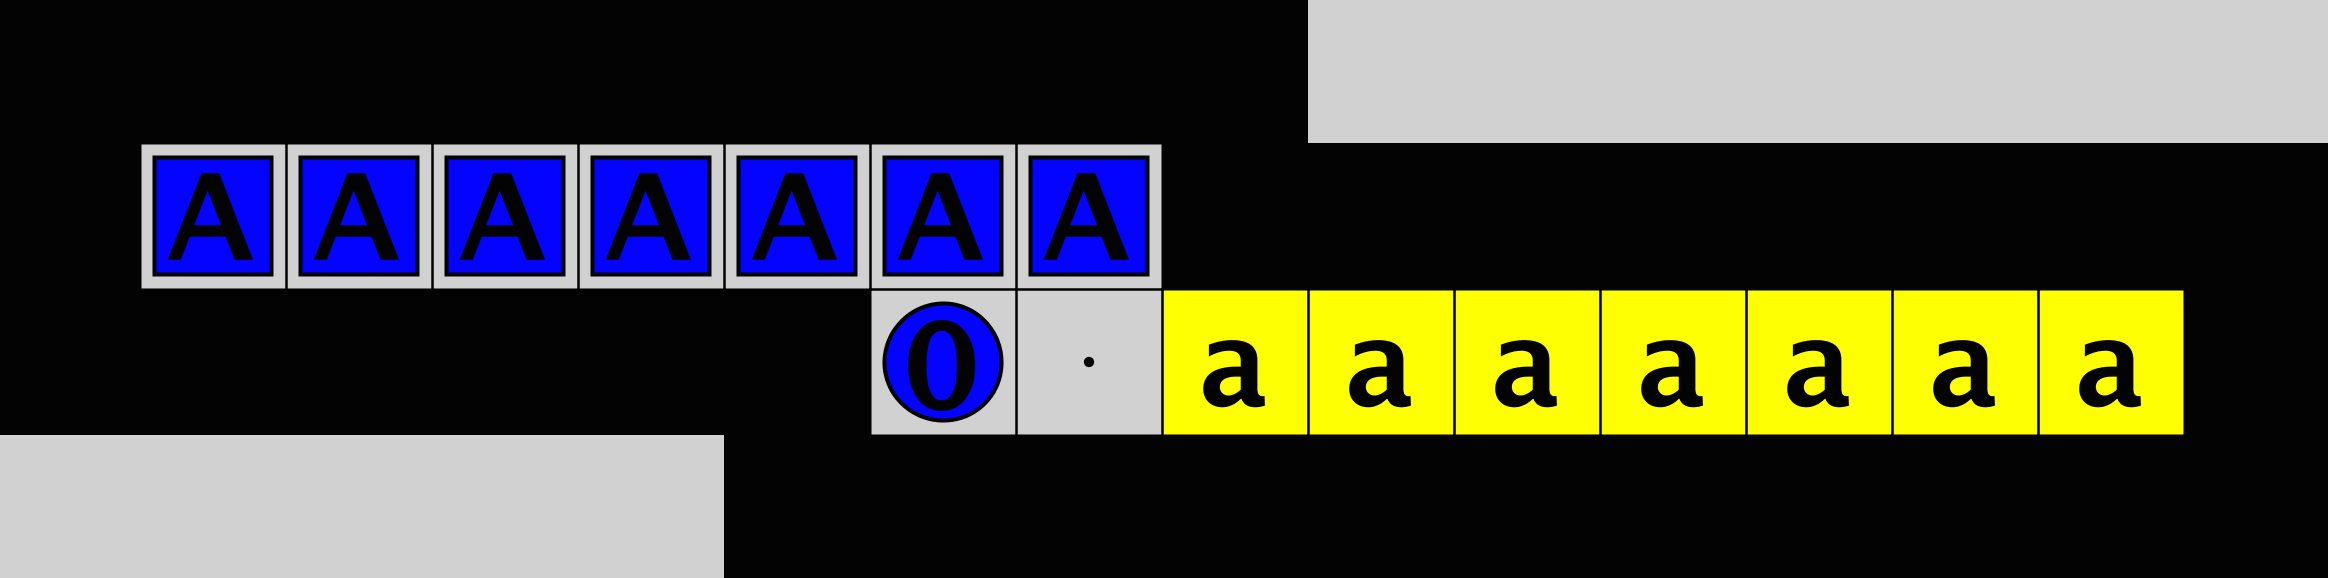
\includegraphics[width=0.3\textwidth]{shortcomings.png}
    \caption{A level where the bidding and choosing of boxes to solve goals with can pose a problem.}
    \label{fig:shortcomings}
\end{figure}

% \begin{verbatim}
% +++++++++
% +AAAAAAA++++++++
% ++++++0 aaaaaaa+
% ++++++++++++++++
% \end{verbatim}


\end{document}
